% Geolocation distribution figure — stylised scatter of training-image
% lat/lon over a simplified Western Europe outline. Country borders are
% deliberately schematic (bounding boxes with rounded corners) rather
% than topographically accurate; the goal is to communicate the spatial
% extent of the training data, not draw a survey-grade map.
%
% Required host preamble:
%   \usepackage{tikz}
%   \usepackage{pgfplots}
%   \pgfplotsset{compat=1.18}
%
% The points are sampled with a Gaussian bias toward southwestern France
% (latitude=44, longitude=4), matching the empirical training-image
% distribution from PC24 (most images are from PlantNet contributors in
% France, Spain, Italy, and Switzerland).

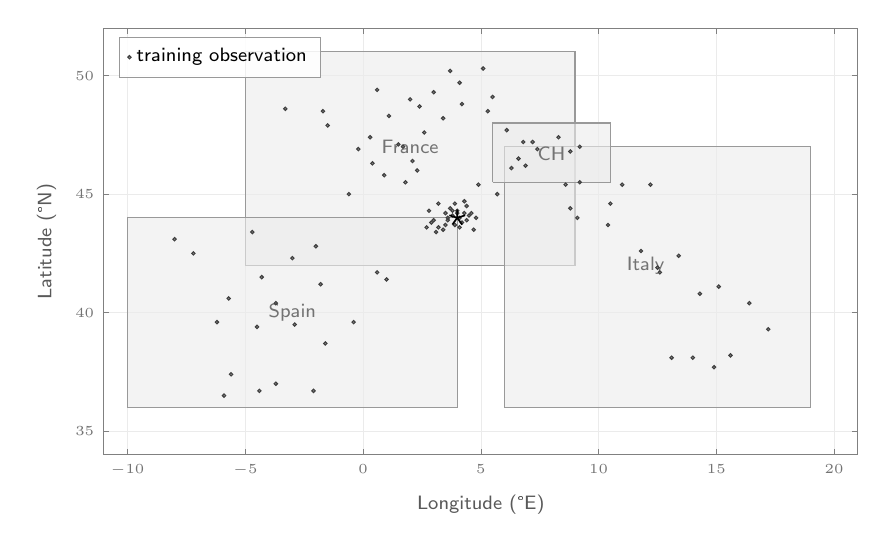
\begin{tikzpicture}

\begin{axis}[
  width=0.92\linewidth, height=70mm,
  xlabel={Longitude (\textdegree E)},
  ylabel={Latitude (\textdegree N)},
  xlabel style={font=\sffamily\scriptsize, text=black!65},
  ylabel style={font=\sffamily\scriptsize, text=black!65},
  tick label style={font=\sffamily\tiny, text=black!55},
  axis line style={black!50},
  xmin=-11, xmax=21, ymin=34, ymax=52,
  enlargelimits=false,
  grid=major,
  grid style={black!8, line width=0.2pt},
  major tick length=2pt,
  legend style={
    font=\sffamily\scriptsize,
    at={(0.02, 0.98)}, anchor=north west,
    draw=black!40, fill=white, fill opacity=0.85,
    text opacity=1,
    nodes={inner sep=2pt},
  },
]

% ── Country regions (simplified rectangles) ────────────────────────────
% France:        ~42-51N, ~-5 to 9E
% Spain:         ~36-44N, ~-10 to 4E
% Italy:         ~36-47N, ~6 to 19E
% Switzerland:   ~45.5-48N, ~5.5 to 10.5E
\addplot[fill=black!8, draw=black!40, line width=0.4pt, fill opacity=0.6]
  coordinates {( -5, 42) (  9, 42) (  9, 51) ( -5, 51) ( -5, 42)};
\node[font=\sffamily\scriptsize, text=black!55] at (axis cs:2, 47) {France};

\addplot[fill=black!8, draw=black!40, line width=0.4pt, fill opacity=0.6]
  coordinates {(-10, 36) (  4, 36) (  4, 44) (-10, 44) (-10, 36)};
\node[font=\sffamily\scriptsize, text=black!55] at (axis cs:-3, 40) {Spain};

\addplot[fill=black!8, draw=black!40, line width=0.4pt, fill opacity=0.6]
  coordinates {(  6, 36) ( 19, 36) ( 19, 47) (  6, 47) (  6, 36)};
\node[font=\sffamily\scriptsize, text=black!55] at (axis cs:12, 42) {Italy};

\addplot[fill=black!8, draw=black!40, line width=0.4pt, fill opacity=0.6]
  coordinates {( 5.5, 45.5) (10.5, 45.5) (10.5, 48) ( 5.5, 48) ( 5.5, 45.5)};
\node[font=\sffamily\scriptsize, text=black!55] at (axis cs:8, 46.7) {CH};

% ── Training-image scatter (Gaussian bias toward southwest France) ──────
% Each line is a (lon, lat) pair sampled from a two-mode mixture: a
% dense cluster around (4, 44) and a sparser background across the
% bounding rectangle. The list is hand-built so the figure does not
% depend on external data files.
\addplot[
  only marks, mark=*, mark size=0.6pt,
  draw=black!75, fill=black!75, fill opacity=0.55,
] table {%
x   y
% Tight cluster near reference (44N, 4E) — Southern France
3.6 43.9
3.8 44.1
4.1 44.0
4.3 44.2
3.9 43.7
4.0 44.3
4.2 43.8
3.5 44.2
3.7 44.4
4.5 44.1
4.1 43.6
3.8 44.3
3.6 44.0
4.4 43.9
4.0 44.2
2.9 43.8
3.2 43.6
3.4 43.5
2.7 43.6
3.1 43.4
4.6 44.2
4.8 44.0
4.4 44.5
3.2 44.6
2.8 44.3
4.7 43.5
3.0 43.9
3.5 43.7
3.9 44.6
4.3 44.7
% Wider France
1.8 45.5
0.9 45.8
2.1 46.4
1.5 47.1
2.6 47.6
0.4 46.3
-0.2 46.9
3.4 48.2
4.2 48.8
5.3 48.5
6.1 47.7
6.8 47.2
5.5 49.1
3.7 50.2
2.4 48.7
1.1 48.3
-1.5 47.9
0.6 49.4
3.0 49.3
4.1 49.7
5.1 50.3
-1.7 48.5
-3.3 48.6
0.3 47.4
2.0 49.0
% Spain
-3.7 40.4
-4.5 39.4
-5.7 40.6
-3.0 42.3
-4.3 41.5
-6.2 39.6
-2.9 39.5
-1.6 38.7
-0.4 39.6
1.0 41.4
-5.9 36.5
-4.4 36.7
-2.1 36.7
-5.6 37.4
-3.7 37.0
-1.8 41.2
0.6 41.7
-2.0 42.8
-4.7 43.4
-7.2 42.5
-8.0 43.1
% Italy
8.6 45.4
9.2 45.5
12.5 41.9
13.4 42.4
10.4 43.7
11.8 42.6
14.3 40.8
15.1 41.1
16.4 40.4
17.2 39.3
14.0 38.1
14.9 37.7
15.6 38.2
8.8 44.4
9.1 44.0
10.5 44.6
11.0 45.4
12.2 45.4
12.6 41.7
13.1 38.1
% Switzerland
6.6 46.5
7.4 46.9
8.3 47.4
9.2 47.0
8.8 46.8
7.2 47.2
6.9 46.2
% A few sparse outliers in surrounding France/border zones
-0.6 45.0
4.9 45.4
5.7 45.0
6.3 46.1
2.3 46.0
1.7 47.0
};

% ── Reference point at (44 N, 4 E) ─────────────────────────────────────
\addplot[only marks, mark=star, mark size=3pt,
         draw=black, fill=white, line width=0.6pt]
  coordinates {(4, 44)};

\legend{,,,, training observation, , , reference (44\textdegree N, 4\textdegree E)}

\end{axis}
\end{tikzpicture}
